\Aufgabe[e]{Isolinien und Isoflächen} {
\begin{abc}
\item Skizzieren Sie (wenn möglich) die Isolinien der folgenden multivariaten Funktionen für die Niveaus 0, 1 und -1:
\begin{iii}
\begin{multicols}{2}
\item $f_1(x,y)=xy,$
\item $f_2(x,y)=x^2y,$
\item $f_3(x,y)=xy^2,$
\item $f_4(x,y)=x^2y^2.$
\end{multicols}
\end{iii}
\item Gegeben ist die Funktion
$$f_5(x,y,z)=x^2+y^2-z.$$
Skizzieren Sie die Schnittpunkte von
\begin{iii}
\item der Ebene $z=0$, $z=1$, $z=-1$ mit ihrer Isofläche mit dem Niveau 1,
\item der Ebene $z=2x+2y$ mit ihrer Isofläche mit dem Niveau -1.
\end{iii}
\end{abc}
}


\Loesung{
\textbf{a)} 
\begin{iii}
\item Die Isolinien von $f_1(x,y) = xy$ sind dargestellt in Abbildung \ref{f_1}.
\item Die Isolinien von $f_2(x,y) = x^2y$ sind dargestellt in Abbildung \ref{f_2}.
\item Die Isolinien von $f_3(x,y) = xy^2$ sind dargestellt in Abbildung \ref{f_3}.
\item Die Isolinien von $f_4(x,y) = x^2y^2$ sind dargestellt in Abbildung \ref{f_4}. 
Es gilt $f_4 \geq 0$, da $f_4$ quadratisch in $x$ und $y$ ist. Daher gibt es keine Isolinie mit dem Niveau -1.
\end{iii}
\begin{figure}[ht]
\begin{center}
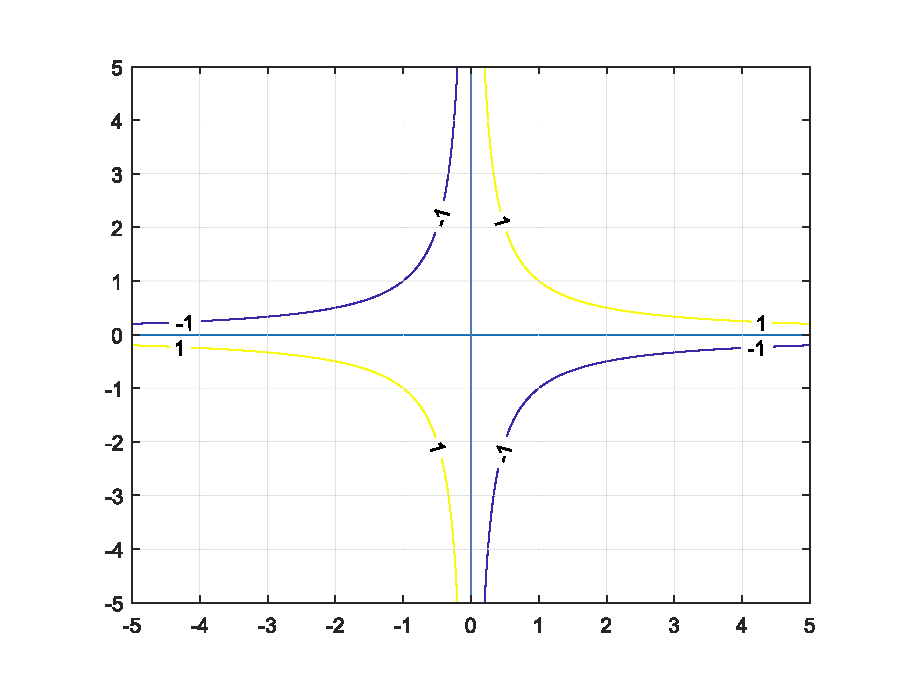
\includegraphics[width=15cm, height=15cm]{../A/analysis/isolines_and_isosurfaces_001_ai.eps}
\caption{Isolinien von $f_1(x,y) = xy$.}
\label{f_1}
\end{center}
\end{figure}

\begin{figure}[ht]
\begin{center}
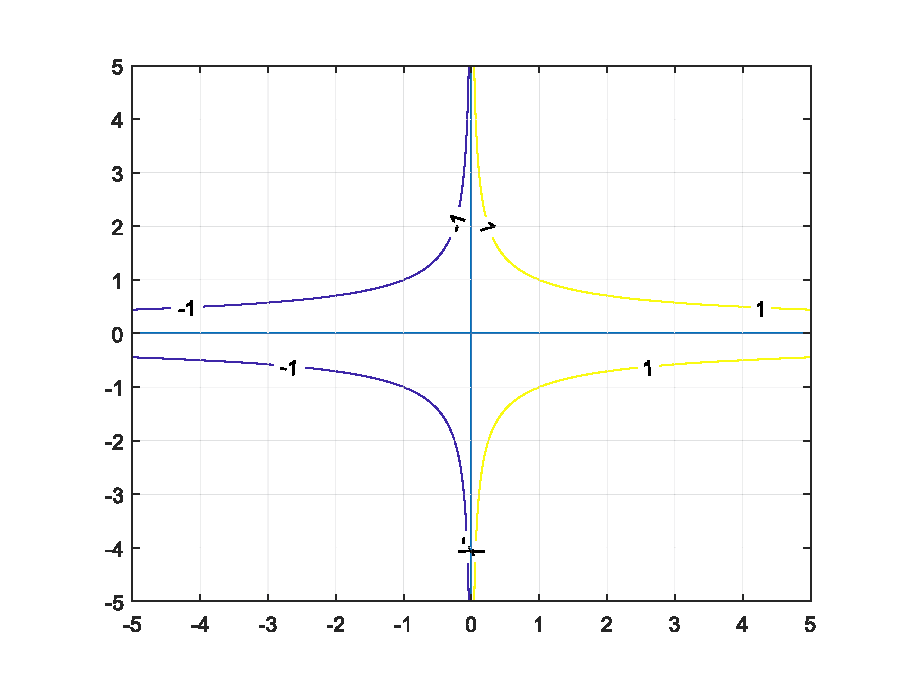
\includegraphics[width=15cm, height=15cm]{../A/analysis/isolines_and_isosurfaces_001_aii.eps}
\caption{Isolinien von $f_2(x,y) = x^2y$.}
\label{f_2}
\end{center}
\end{figure}

\begin{figure}[ht]
\begin{center}
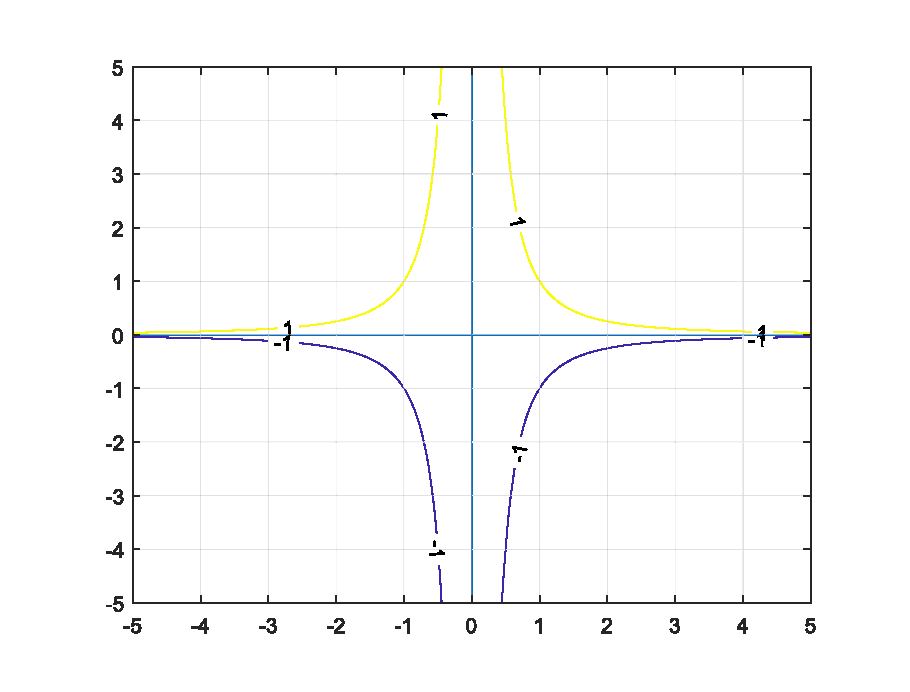
\includegraphics[width=15cm, height=15cm]{../A/analysis/isolines_and_isosurfaces_001_aiii.eps}
\caption{Isolinien von $f_3(x,y) = xy^2$.}
\label{f_3}
\end{center}
\end{figure}

\begin{figure}[ht]
\begin{center}
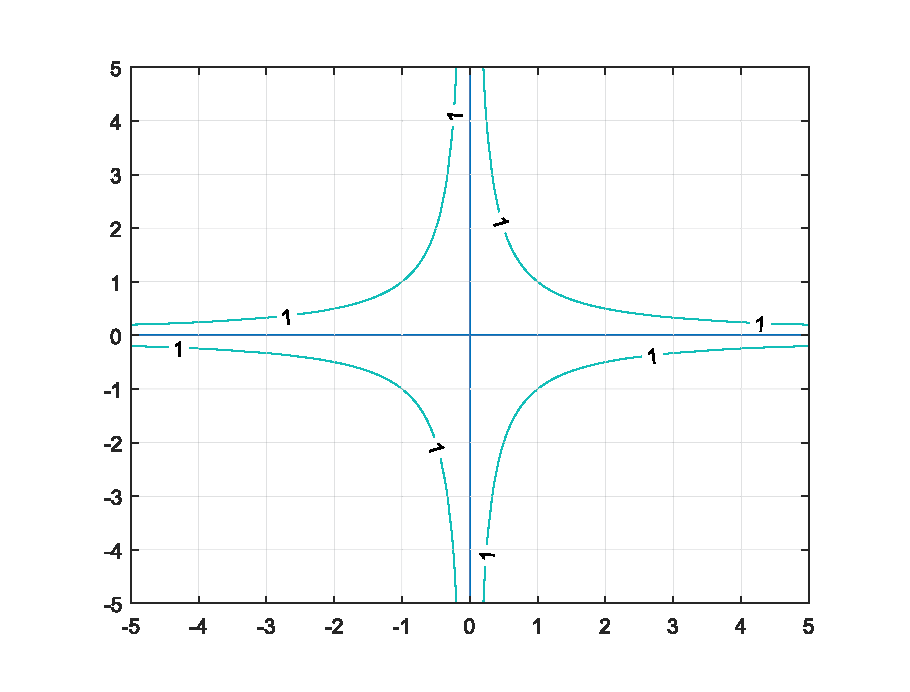
\includegraphics[width=15cm, height=15cm]{../A/analysis/isolines_and_isosurfaces_001_aiv.eps}
\caption{Isolinien von $f_4(x,y) = x^2y^2$.}
\label{f_4}
\end{center}
\end{figure}


\textbf{b)}
\begin{iii}
\item Die Funktion $f_5$ ist ein Paraboloid. Der Schnittpunkt mit der Ebene $z = 0$ ist ein Kreis mit dem Radius 1 (siehe Abbildung \ref{z=0}).\\
Der Schnittpunkt mit der Ebene $z = 1$ ist ein Kreis mit dem Radius $\sqrt{2}$ (siehe Abbildung \ref{z=1}). 
Der Schnittpunkt mit der Ebene $z = -1$ ist der Punkt bei $(0,0)$ (siehe Abbildung \ref{z=-1}). 
\item Der Schnittpunkt der Funktion $f_5$ mit der Ebene $z =2x+2y$ ist eine Ellipse (siehe Abbildung \ref{z=2x+2y}).
\end{iii}
\begin{figure}[ht]
\begin{center}
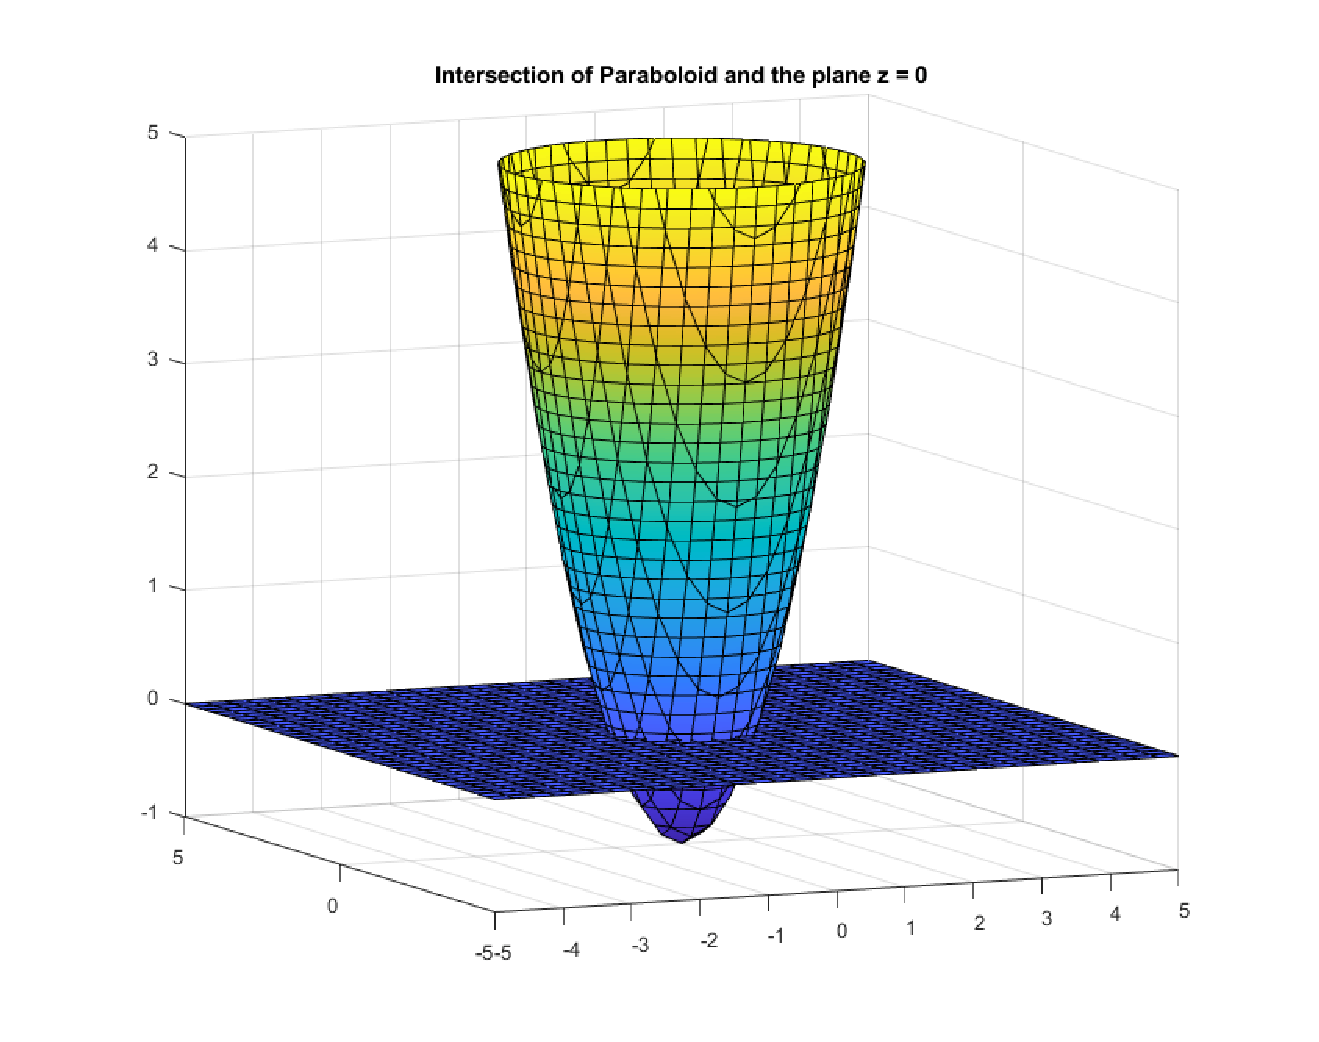
\includegraphics[width=15cm, height=15cm]{../A/analysis/isolines_and_isosurfaces_001_bi1.eps}
\caption{Schnitt des Paraboloiden mit der Ebene $z=0$.}
\label{z=0}
\end{center}
\end{figure}

\begin{figure}[ht]
\begin{center}
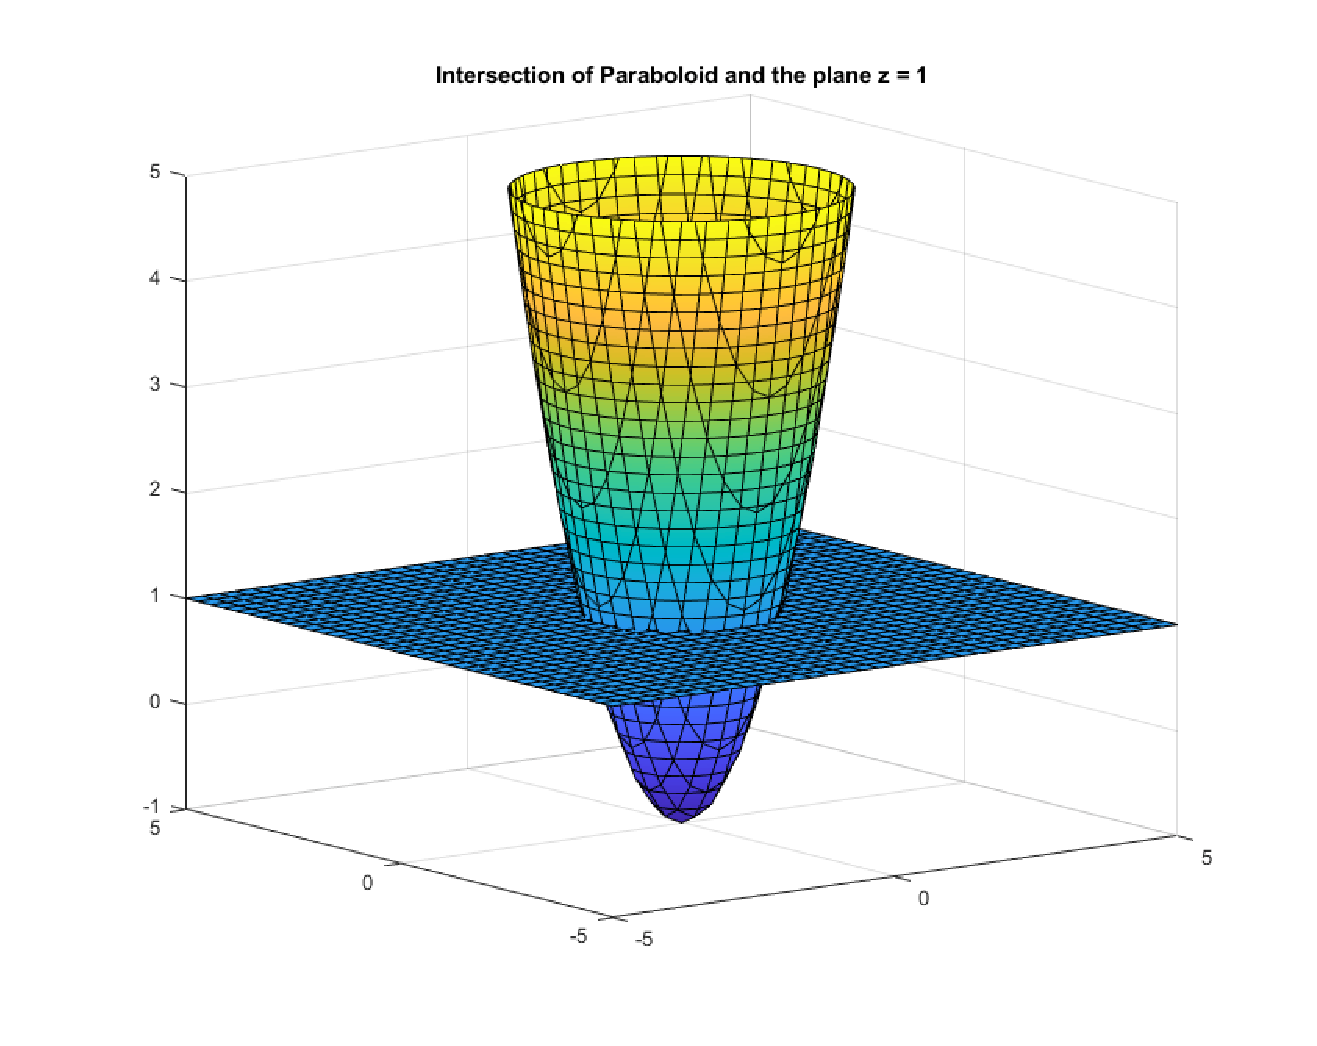
\includegraphics[width=15cm, height=15cm]{../A/analysis/isolines_and_isosurfaces_001_bi2.eps}
\caption{Schnitt des Paraboloiden mit der Ebene $z=1$.}
\label{z=1}
\end{center}
\end{figure}

\begin{figure}[ht]
\begin{center}
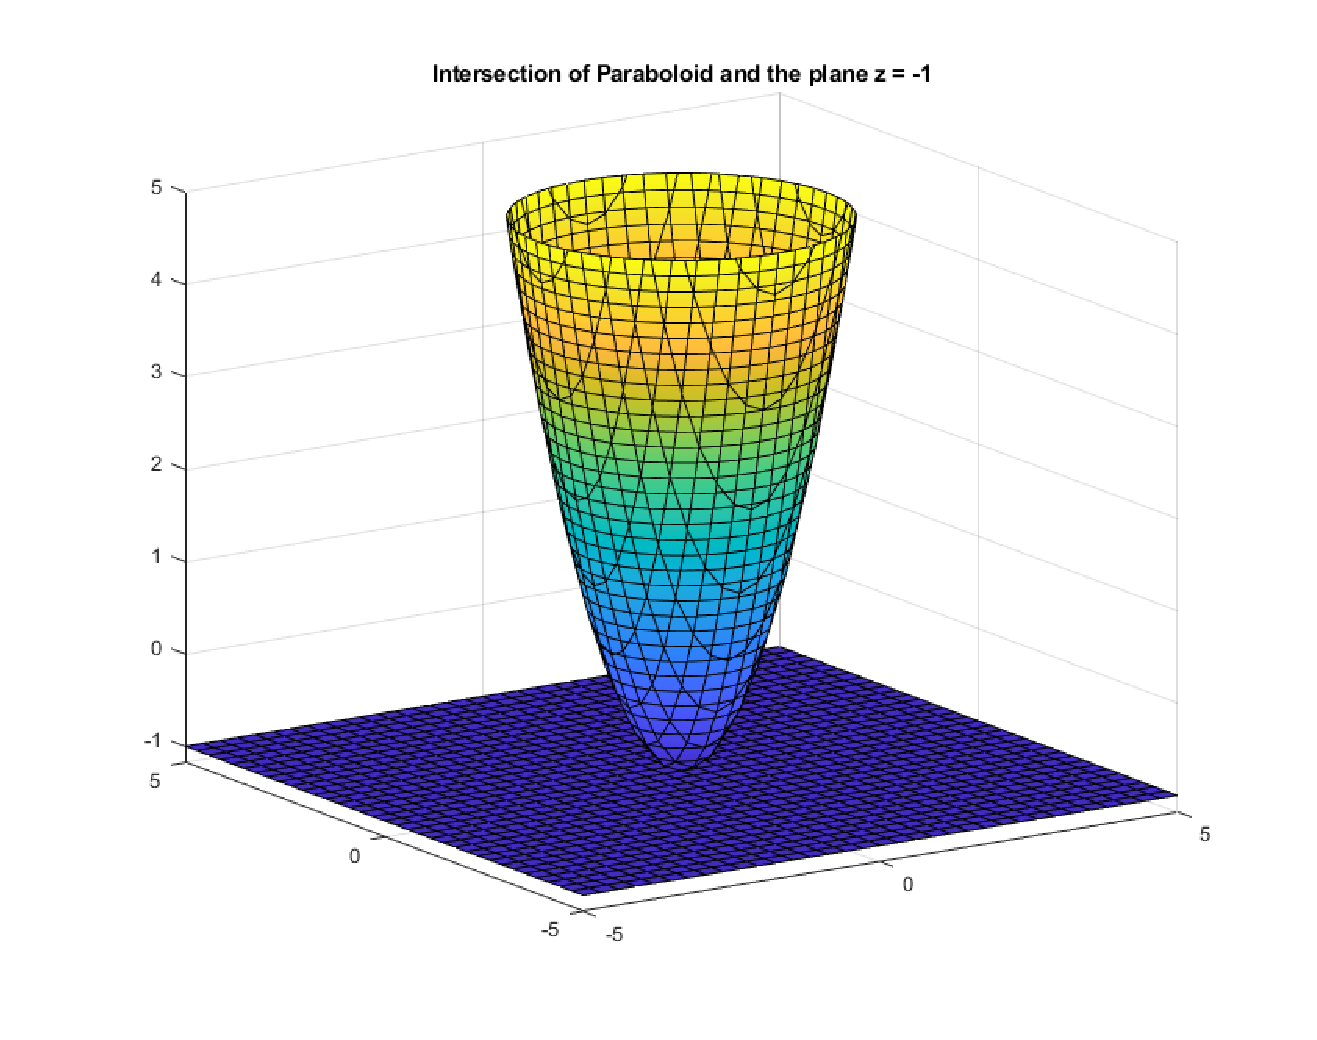
\includegraphics[width=15cm, height=15cm]{../A/analysis/isolines_and_isosurfaces_001_bi3.eps}
\caption{Schnitt des Paraboloiden mit der Ebene $z=-1$.}
\label{z=-1}
\end{center}
\end{figure}

\begin{figure}[ht]
\begin{center}
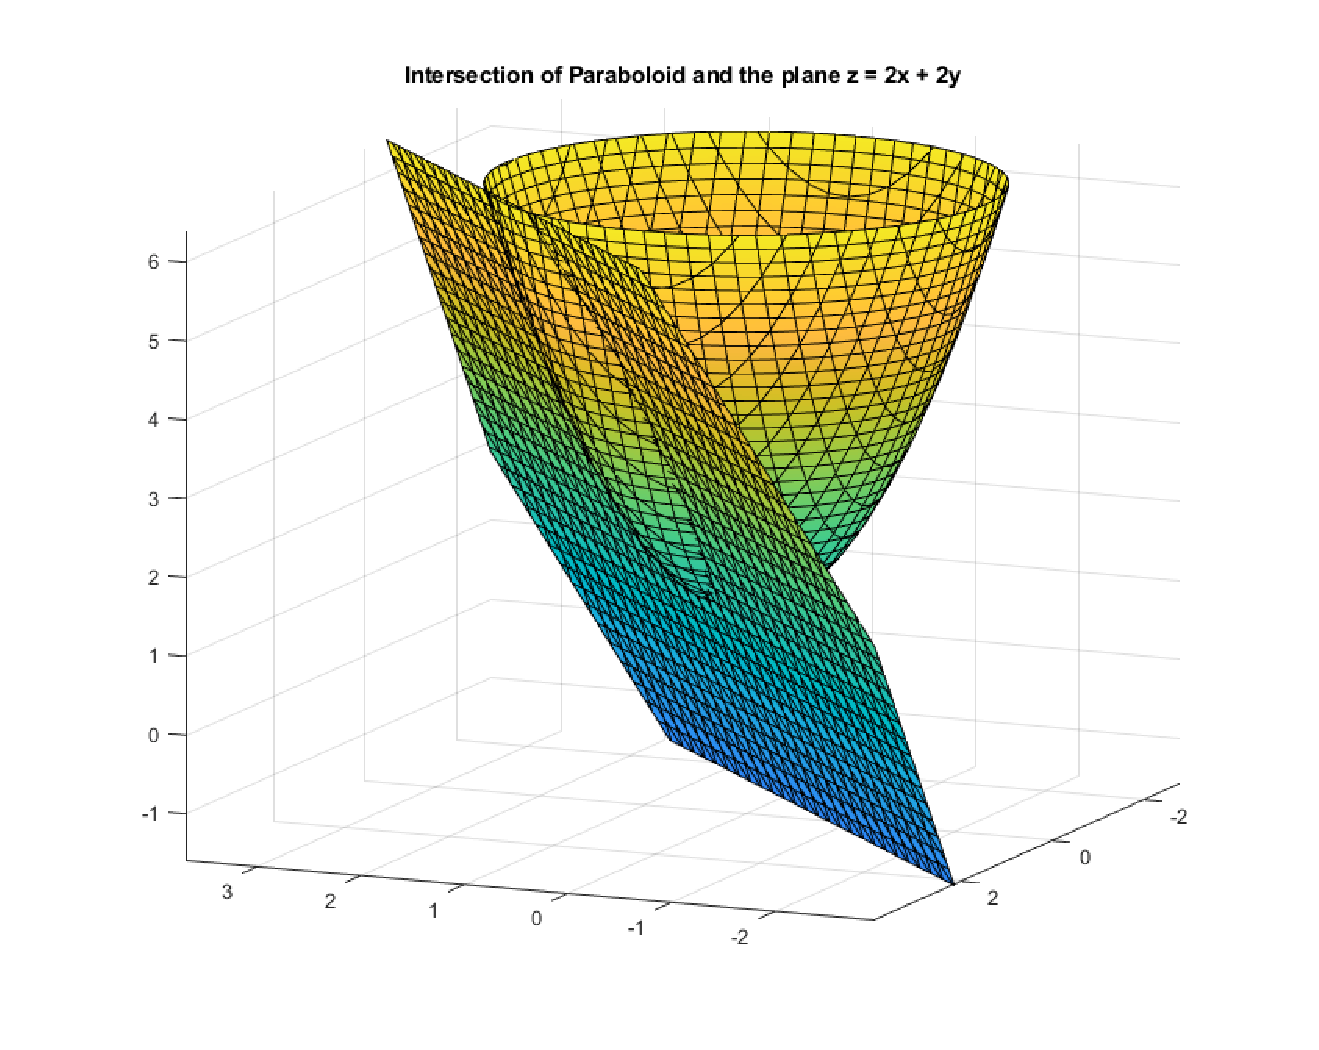
\includegraphics[width=15cm, height=15cm]{../A/analysis/isolines_and_isosurfaces_001_bii.eps}
\caption{Schnitt des Paraboloiden mit der Ebene $z=2x+2y$.}
\label{z=2x+2y}
\end{center}
\end{figure}


}

